\documentclass[a4paper, 12pt, hidelinks]{article}

\title{Honours Project Dissertation}
\author{Joe Barrett}

\usepackage[natbibapa]{apacite}
\bibliographystyle{apacite}
\usepackage{blindtext}
\usepackage{booktabs}
\usepackage[ddmmyyyy]{datetime}
\usepackage{eurosym}
\usepackage{fancyhdr}
\usepackage{fontspec}
\usepackage[margin=1in]{geometry}
\usepackage[toc,acronym]{glossaries}
\usepackage{graphicx}
\usepackage{hyperref}
\usepackage[none]{hyphenat}
\usepackage[table]{xcolor}
\usepackage{url}

\setmainfont{Arial}

\pagestyle{fancy}
\renewcommand{\headrulewidth}{0pt}

\lhead{Joe Barrett - 40117680}
\rhead{SOC10101 Honours Project}
\cfoot{\thepage}

\makeglossary
\loadglsentries{glossary}

\begin{document}
	\begin{titlepage}
	\begin{center}
		
		\vspace*{3cm}
		{\LARGE Calculation of Mountain Bike Suspension Settings through Image Analysis}
		
		\vspace{3cm}
		{\large Joe Barrett - 40117680}

		\vfill
		Submitted in partial fulfilment of the requirements of Edinburgh Napier University for the Degree of BEng (Hons) Software Engineering
		
		\vspace{1cm}
		School of Computing
		
		\vspace{1cm}
		\today
	\end{center}
\end{titlepage}
	\begin{abstract}
		\blindtext
	\end{abstract}
	\newpage
	\tableofcontents
	\newpage
	\listoftables
	\newpage
	\listoffigures
	\newpage
	\section{Introduction}
	\subsection{Context}
	A survey carried out by the International Mountain Bike Association shows the average price of mountain bikes owned in Europe to be \euro2546 (\pounds2206) \citep{imbasurv}. Starting at around \pounds1000 \citep{giantstance}, enthusiast level mountain bikes can be purchased with suspension for both the front and rear wheels, known as \gls{fs} bikes. Even at this comparably low cost, the suspension units have multiple adjustments available to tune and personalize how they operate.
	\\\\
	To ensure the \gls{fork} and \gls{shock} function correctly they must be set up for the rider's weight and intended use of the bike. As this is considered a specialist area, many entry and mid level riders will lack the knowledge of this process or be unsure of how the suspension should operate meaning the rider could use the bike without the suspension set up correctly.
	\\\\
	It has been proven that using a \gls{fs} over a \gls{ht} offers a performance advantage to the rider \citep{fullsusperf}. However if the suspension fork and/or shock have not been set up, it can be detrimental to the rider's performance and potentially lead to injury. For example, if a shock has too little \gls{rebounddamping} set and the rider goes off a jump, the excessive speed at which the rear of the bike extends can create forwards rotation, causing the rider to go over the handlebars of the bike.
	\\\\
	Additionally, an incorrect suspension setup can cause excessive wear and tear on the bike's frame and components. Suspension which is set too soft can allow for bottoming out which expends excess forces into the frame and potentially cracks the frame's structure. Suspension set too hard forces energy, which it would normally soak up, into the wheels and tires causing denting and warping of the wheel rims.
	\\\\
	Many bicycle retailers will set up the suspension on a newly purchased mountain bike for the customer on delivery. Most of the time this will be enough to avoid incident but due to the extra weight of the equipment riders use, i.e. helmet, hydration pack, body armor which the customer will not be wearing at the time of delivery, this setup is regularly inaccurate. Furthermore, with some manufacturers choosing direct sales over local retailers \citep{roseonline, ytonline}, this setup can be circumnavigated altogether.
	\\\\
	Since the birth of the modern smartphone in 2007 brought along by the first generation Apple\textregistered\ iPhone\textregistered\ and introduction of the Android\texttrademark\ mobile operating system, the use of mobile computing in everyday life has grown rapidly. Google\texttrademark\ stated that there were approximately 1.4 active Android users worldwide in 2015 \citep{androidusers}.
	\\\\
	The introduction of activity tracking devices and mobile applications such as FitBit \citep{fitbit} and Strava \citep{strava} and their growing popularity \citep{apppopularity} shows that individuals are welcome to the idea of using smartphones to aid or augment their participation in hobbies or sports. Due to this popularity and in a bid to give every rider the ability to setup and tune their own suspension, either at home or while out on a ride, companies have set about producing small devices \citep{sussmybike, shockwiztrademark} and mobile applications \citep{foxird} which aid riders in the process.
	
	\subsection{Mountain Bike Suspension Concepts}
		The purpose of suspension on a mountain bike is to divert energy from bumps and rough features in a trail away from the rider to improve comfort and  performance by maintaining contact between the tires and the ground. This requires the use of a spring and damper, collectively known as a shock absorber, which allows the wheel to move away from the feature when it makes contact and make a controlled return once it has been passed.
	\subsubsection{Travel and Stroke} 
		Travel is the distance which the bike's fork or frame allow the wheel to move in and upward direction. Stroke is the distance that the shock absorber can compress before it bottoms out. Travel is measured in inches or millimeters and can range from 80mm to 210mm. The amount of travel which a bike has normally denotes which discipline it was intended for. Typically less suspension is required for endurance oriented riding and more for aggressive and rough situations.
		\begin{table}[h!]
		\centering
		\caption{Table of common suspension travels and intended disciplines}
		\label{tab:table1}
		\begin{tabular}{|c|cccc|}
			\hline
			Travel (mm)&Cross Country&Trail&Enduro&Downhill\\
			\hline
			80&\cellcolor[gray]{0.5}&&&
			\\
			100&\cellcolor[gray]{0.5}&&&
			\\
			120&\cellcolor[gray]{0.5}&\cellcolor[gray]{0.5}&&
			\\
			140&&\cellcolor[gray]{0.5}&\cellcolor[gray]{0.5}&
			\\
			160&&&\cellcolor[gray]{0.5}&
			\\
			180&&&\cellcolor[gray]{0.5}&\cellcolor[gray]{0.5}
			\\
			+200&&&&\cellcolor[gray]{0.5}\\
			\hline
		\end{tabular}
	\end{table}
	\subsubsection{Front Suspension}
		Front suspension commonly employs a linear telescoping shock absorber, known as a fork due to it's dual sided construction. On nearly all suspension forks the stroke of the shock is 1:1 with the potential travel of the wheel. Front suspension is found on all \gls{fs} and \gls{ht} bikes.
	\subsubsection{Rear Suspension}
		Rear suspension uses a shock absorber much smaller than a fork and does not operate on a 1:1 ratio. Bike frames incorporate one or more pivot points and linkages which allows the wheel to move and act as multipliers for the suspension. Rear ratios are expressed as n:1 where n is the distance the rear wheel moves for every 1mm the shock compresses through its stroke. This is the average leverage ratio.  
		\\\\
		As all rear suspension designs are different and the rear wheel must rotate around the main pivot as opposed to moving linearly, the frame will behave differently through its travel and depending on the type of shock it is using. Because of this the average ratio is normally dismissed in favour of a leverage curve.
		\begin{figure}[h!]
			\centering
			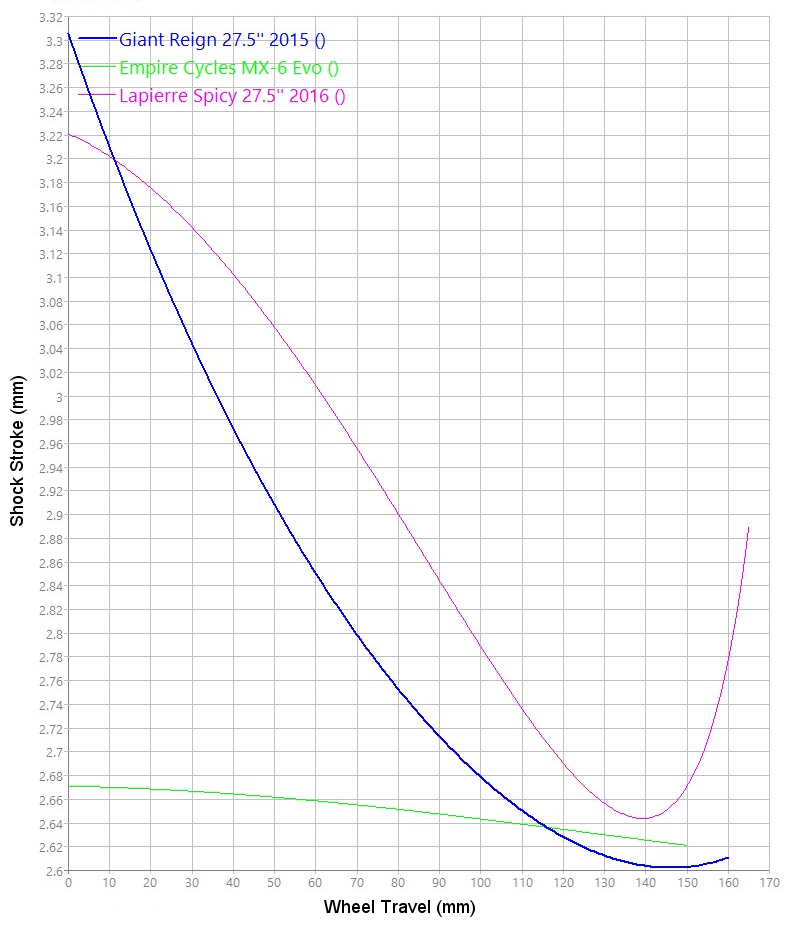
\includegraphics[width=10cm]{../images/3_bike_lev_ratio.jpg}
			\caption{Leverage curves of three modern suspension designs}
			\label{fig:3_bike_lev_ratio}
		\end{figure}
		\\\\
		Figure \ref{fig:3_bike_lev_ratio} shows the leverage curves of three modern suspension designs. Each of these designs has between 150mm and 170mm of travel and uses the 27.5 inch wheel size however it can be seen that their suspension hosts drastically different characteristics. 
		\\\\
		The Virtual Pivot Point design of the Giant Reign (shown blue) has a initial falling rate, meaning the shock can be compressed easily, but slows down and even rises slightly towards the end of its travel. This means the suspension will feel soft most of the time but feel stiffer on large compressions. This is emphasised by the Horst Link system of the Lapierre Spicy (shown magenta) which has a large rise at the end of its travel.
		\\\\
		In contrast, the curve of the Single Pivot Empire MX-6 Evo (shown green) is considered linear. This is due to the MX-6 having only one pivot and swinging arm, as opposed to multiple pivots and linkages of the VPP and Horst designs, so there is an almost direct input from the rear wheel to the shock.
	\subsubsection{Damping}
	\paragraph{Compression Damping}
		
	\paragraph{Rebound Damping}
	\newpage
	\section{Literature Review}
	\newpage
	\section{Approach}
	\newpage	
	\section{Results}
	\newpage
	\section{Critical Evaluation}
	\newpage
	\section{Conclusion}
	\newpage
	\bibliography{bibliography}	
	\newpage
	\printacronyms
	\printglossary[type=main]
	
\end{document}